\chapter{Application to a dynamically twisted null point}
\label{chp:null_point_khi}

\graphicspath{{images/null_point_khi/}}

\section{Introduction}

This chapter presents the results of a series of numerical experiments intended to develop an understanding of the effect of anisotropic viscosity on the Kelvin-Helmholtz instability (KHI) in the fan plane of a magnetic null point, reproducing and extending the work of Wyper \& Pontin~\cite{wyperKelvinHelmholtzInstabilityCurrentvortex2013}. The numerical experiment takes the form of the dynamic twisting of an initially static magnetic null point at the footpoints of its spines, resulting in a current-vortex sheet forming in the fan plane which, given appropriate parameter choices, can be unstable to the KHI. In the course of twisting the null point, it is discovered that continued driving past the point at which the KHI occurs causes the null to spontaneously undergo spine-fan reconnection and collapse. The evolution of the KHI and the eventual collapse of the null is found to depend strongly on the form of viscosity.

The KHI has been well studied in MHD (see~\cite{faganelloMagnetizedKelvinHelmholtz2017} for a recent review and~\cite{chandrasekharHydrodynamicHydromagneticStability1981} for the classical treatment) and has been found in a number of coronal contexts, both in numerical simulations~\cite{howsonEffectsResistivityViscosity2017,wyperKelvinHelmholtzInstabilityCurrentvortex2013} and in observations~\cite{foullonMAGNETICKELVINHELMHOLTZINSTABILITY2011,yangObservationKelvinHelmholtz2018}.  In general, the effect of a magnetic field is stabilising; when the wavevector of a perturbation in a shear layer is parallel or at an oblique angle to a magnetic field, magnetic tension acts to stabilise the KHI~\cite{chandrasekharHydrodynamicHydromagneticStability1981,ryuMagnetohydrodynamicKelvinHelmholtzInstability2000}. Otherwise, the KHI acts as an interchange instability and the magnetic field does not affect its linear stability~\cite{chandrasekharHydrodynamicHydromagneticStability1981}.

In the case where a velocity shear coincides with a magnetic shear, forming a current-vortex sheet, the balance of shear layer strengths and thickness dictates if the KHI, tearing instability, or some mixture, is excited. Generally, when the magnetic shear is strong compared to the velocity shear, the KHI is suppressed and the tearing instability grows~\cite{einaudiResistiveInstabilitiesFlowing1986}. The nonlinear development of the KHI is known to enhance reconnection by local distortion of magnetic field lines and generation of current sheets~\cite{minEffectsMagneticReconnection1997} and by generating local turbulence in conjunction with the tearing instability~\cite{kowalKelvinHelmholtzTearingInstability2020}.

The effect of (anisotropic) viscosity on the stability of a current-vortex sheet is to suppress the growth of the KHI, although viscosity is found to enhance the linear growth of the tearing instability, where the KHI is stabilised by a strong magnetic field~\cite{einaudiResistiveInstabilitiesFlowing1989}. A number of studies suggest isotropic viscosity can also slow and even suppress the KHI~\cite{howsonEffectsResistivityViscosity2017,roedigerViscousKelvinHelmholtzInstabilities2013a,wyperKelvinHelmholtzInstabilityCurrentvortex2013}.

Magnetic null points, locations in a magnetic field where the field strength goes to zero, are an abundant feature in the topologically complex coronal magnetic field~\cite{edwardsNullPointDistribution2015}. Given that they are sites coinciding with changes in topology, they are strongly associated with reconnection processes~\cite{yangImagingSpectralStudy2020,sunHOTSPINELOOPS2013}. Additionally they are inferred to participate in a number of high-energy phenomena such as in the generation of flare ribbons in compact solar flares~\cite{massonNATUREFLARERIBBONS2009,pontinWhyAreFlare2016a}, production of jets~\cite{moreno-insertisPLASMAJETSERUPTIONS2013} and of coronal mass ejections (CMEs)~\cite{barnesRelationshipCoronalMagnetic2007,zouContinuousNullPointMagnetic2020}, particularly through their necessary involvement in the breakout model of eruptive solar flares~\cite{macleanTopologicalAnalysisMagnetic2005}.

A well studied form of reconnection in 3D null points is spine-fan reconnection, where a strong current sheet forms in the vicinity of the null point and enables efficient reconnection between the magnetic field making up the spine and fan plane, collapsing the field around the null in the process~\cite{thurgoodImplosiveCollapseMagnetic2018}. The collapse of a null point has the potential to develop into a form of oscillatory reconnection~\cite{thurgoodThreedimensionalOscillatoryMagnetic2017}.

The layout of this chapter is as follows. The numerical setup of the simulations is presented in Section~\ref{sec:khi_numerical_setup}, including a description of the model of linear null point and the driver used. The methods of calculating the stability measures, shear layer properties and reconnection rate are described in Section~\ref{sec:khi_analysis}. In the first part of Section~\ref{sec:khi_results} the results of a high-resolution pair of simulations are presented for a single choice of viscosity and resistivity parameters and the effect of the viscosity model compared. In the second part, the results of a parameter study are presented, generalising the high-resolution results. The chapter concludes with a discussion of findings in Section~\ref{sec:khi_discussion} and conclusions in Section~\ref{sec:khi_conclusions}.

\section{Numerical setup}

\label{sec:khi_numerical_setup}

The magnetic structure of the null point with the spine aligned along the $z$-axis is written in non-dimensional units as
\begin{equation}
  \label{eq:null_point_field}
  \vec{B} = (x, y, -2z).
\end{equation}
The non-dimensionalisation scheme is identical to that used in chapter~\ref{chp:kink_instability}. The domain is a box of dimension $[-3.5, 3.5]\times[-3.5, 3.5]\times [-0.25, 0.25] $ in the $x$, $y$ and $z$ directions, respectively. The initial velocity is uniformly zero, the initial density is uniformly $\rho = 1$ and the internal energy is uniformly $\varepsilon = 5/4$, corresponding to a temperature of $1.44 \times 10^9$K and a plasma beta of $\beta \approx 0.017$.

\begin{figure}[t]
  \centering
      \includegraphics[width=0.5\linewidth]{field_line_plots/cropped/v-4r-4-isotropic_0008_cropped.png}
  \caption{Field lines at $t=4$ with start points anchored at a radius of $0.05$ around the spine, with the magnitude of the velocity driver shown as a slice. At this time the driver has reached its final maximum velocity of $u_0 = 0.5$. The spines of the null point already show an appreciable degree of twist.}%
  \label{fig:field_line_plots/v-4r-4-iso-field-8}
\end{figure}

The velocity driver at the upper and lower boundaries is of an identical functional form to that used in chapter~\ref{chp:kink_instability_straight} but with modified driver parameters of $u_0 = 0.09$, $u_{r0} = 5.56$, $t_r = 0.25$ and $r_d = 36$. The peak velocity after the ramping time is $u_0$. The driver twists the footpoints of the upper and lower spines of the null point, dragging the field and introducing twist throughout the entire null point (figure~\ref{fig:field_line_plots/v-4r-4-iso-field-8}). This field and driver is similar to the setup of Wyper and Pontin~\cite{wyperKelvinHelmholtzInstabilityCurrentvortex2013}.

Unlike previous chapters, here the Braginskii-inspired parallel function~\ref{eq:alt_switching1} is used with the general switching model~\ref{eq:switching_model} to avoid the numerical cut-off associated with the spline representation of the von Mises function~\ref{eq:switching_function}. In tests it was found that the sharp transition where the von Mises function transitions to fully anisotropic (see section~\ref{sec:switching_function}) was exciting a small perturbation and disrupting the results. The parallel Braginskii switching function does not suffer from this issue.

The main parameter study required 18 simulations to be run in total; one per viscosity model for each of the 9 parameter choices. As a result a relatively low resolution of $320$ grid points in each direction is used for these runs. A higher resolution pair of simulations were run for each viscosity model at the resolution of $640$ grid points. As well as forming the basis for a detailed analysis, these higher-resolution simulations provide evidence that the lower resolution simulations have suitably converged.

\section{Tools of analysis}

\label{sec:khi_analysis}

\subsection{Shear layer properties}

To quantify the differences between the shear layers produced using different viscosity models, the peak vorticity and current density within the current-vortex sheets are measured, along with the radii at which the peaks occur. These radii are then used as the locations at which the absolute difference in azimuthal velocity $\Delta u$ and magnetic field $\Delta B$ across the shear layers are measured, calculated as the difference between the maximum and minimum values of velocity or magnetic field either side of the shear layer. The distance between the maximum and minimum points gives a measurement of the thickness of the shear layers, $L_u$ and $L_B$. These measures are all used in the calculation of the stability measures discussed in the proceeding section.

\subsection{Stability measures}

\label{sec:stability_measures}

Following Wyper and Pontin~\cite{wyperKelvinHelmholtzInstabilityCurrentvortex2013}, two quantities are used in understanding the stability of the current-vortex sheet: the fast mode Mach number $M_f$, associated with the shear in velocity, and a parameter $\Lambda$ describing the balance of stability between the tearing mode and the KHI in a current-vortex sheet. The fast mode Mach number is given by
\begin{equation}
  \label{eq:mach_numbers}
  M_f = \frac{\Delta u}{\sqrt{c_s^2 + c_A^2}}
\end{equation}
where $c_s$ and $v_A$ are the local sound and Alfv\'en speeds, respectively. The parameter $\Lambda$ is given by
\begin{equation}
  \label{eq:khi_stability_param}
  \Lambda = \frac{L_b}{L_u} M_A^{2/3},
\end{equation}
where $M_A$ is the projected Alfv\'en Mach number
\begin{equation}
  \label{eq:alfven_mach_number}
M_A = \frac{\Delta u \sqrt{\rho}}{\Delta B}.
\end{equation}
Since the shear layer occurs in the presence of a guide field (that of the initial magnetic null point) which is not included in the linear stability study of the KHI, the difference in magnetic field $\Delta B$ is used in the Alfv\'en Mach number as opposed to the full magnetic field strength $|\vec{B}|$. In this way the Alfv\'en Mach number can be considered projected on to the shear layer. 

Plotting the radial dependence of these quantities over the shear layers gives an idea of the probable stability based on the stability analysis performed by~\cite{einaudiResistiveInstabilitiesFlowing1986}. That analysis predicts that a current-vortex sheet will be unstable to the KHI when $M_f < 2$ and $\Lambda > 1$. When $\Lambda < 1$, the analysis predicts that the sheet should be unstable instead to the tearing instability. It should be noted that the analysis of~\cite{einaudiResistiveInstabilitiesFlowing1986} is 2D and does not include the effect of viscosity. The presence of viscosity and the 3D guide field in the system studied here require us to use their stability criteria only as approximations.

\subsection{Reconnection rate}

The reconnection rate is calculated using the same method employed in chapter~\ref{chp:kink_instability}. In summary, the reconnection rate local to a given magnetic field line is calculated as the local parallel electric field (that is, parallel to the magnetic field) integrated along the field line. By choosing a grid of starting points and integrating along each associated field line, we construct an image of reconnection rates projected onto the grid of field line seed points. This is used to explore the spatial distribution of reconnection. The maximum value across all seed points gives the accepted measure of reconnection rate, the maximum integrated value~\cite{galsgaardSteadyStateReconnection2011,priestNatureThreedimensionalMagnetic2003,schindlerGeneralMagneticReconnection1988}.

\section{Results}

\label{sec:khi_results}

In the first part of the results, the evolution of the high-resolution pair of simulations is presented, both performed using a resistivity of $\eta = 10^{-4}$ and viscosity $\nu = 10^{-4}$, and the effect of the two viscosity models are compared. These simulations capture the main features of the response to the driver: the formation of a current-vortex sheet in the fan plane, the appearance of counterflows, the (potential) growth of a KHI, and an eventual null collapse. This specific choice of parameters also highlights the differences between the isotropic and the switching viscosity models, mainly the suppression of the KHI in the isotropic case, and the quicker collapse of the null in the switching case. These results are then generalised to other parameter choices in the proceeding section.

\subsection{Evolution of a typical case}
\label{sec:null_point_khi_single_case}

The evolution of the high-resolution, typical cases is detailed in stages, first exploring the formation, stability and breakup of the current-vortex sheet, before investigating the collapse of the null. Then, the evolution is summarised through an analysis of the energy budget and reconnection rate in time.

\subsubsection{Formation of the current-vortex sheet}

\begin{figure}[t]
  \centering
    \begin{tabular}[t]{cc}
    %\hline
    \begin{subfigure}{0.49\textwidth}
      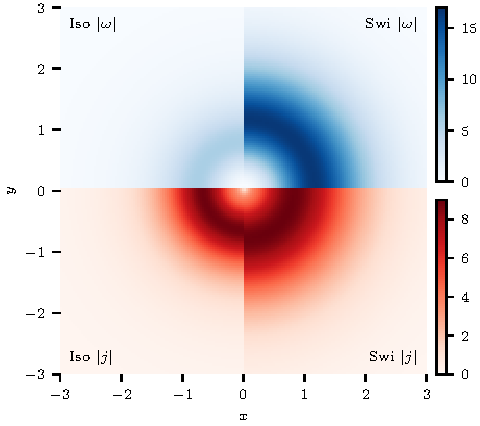
\includegraphics[width=\linewidth]{v-4r-4_vorticity_current_ring_t_3}
      \caption{Vorticity and current density rings.}
      \label{fig:v-4r-4_vorticity_current_ring_t_3}
    \end{subfigure}
    %&
    %\begin{tabular}{c}
    %\smallskip
    %\begin{subfigure}{0.49\textwidth}
      %\includegraphics[width=\linewidth]{v-4r-4_counterflows_t_3}
      %\caption{Azimuthal velocity}
      %\label{fig:v-4r-4_counterflows_t_3}
    %\end{subfigure}
    %\\
    %\begin{subfigure}{0.49\textwidth}
      %\includegraphics[width=\linewidth]{v-4r-4_lorentz_counterflows_t_3}
      %\caption{Azimuthal component of Lorentz force}
      %\label{fig:v-4r-4_lorentz_counterflows_t_3}
    %\end{subfigure}

    \begin{subfigure}{0.49\textwidth}
      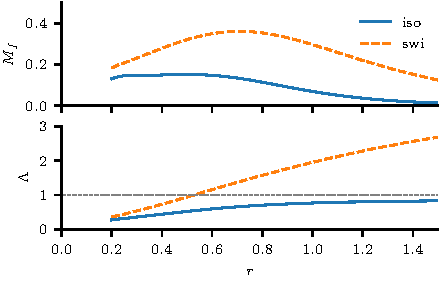
\includegraphics[width=\linewidth]{v-4r-4_mach_t_6}
      \caption{Stability parameters}%
      \label{fig:v-4r-4_mach_t_6}
    \end{subfigure}
    \end{tabular}\\
%\hline
    \end{tabular}
\caption{Vorticity $|\omega|$ and current density $|j|$ rings and the velocity and Lorentz forces associated with the counterflows. The switching model permits rings of greater radial extent and notably stronger vorticity. Azimuthal flows counter to the relevant driver are accelerated due to the action of the magnetic tension force. All figures present data at $t=3$. Figures (b) and (c) are sliced through $x$ and show both isotropic (left of each image) and switching (right of each image) results.}
\label{fig:rings_and_counterflows}%
\end{figure}

Initially, the torsional Alfv\'en waves injected by the driver trace the field surrounding the null, moving first down the spines then out along the fan plane. This occurs from above and below. The upper and lower waves eventually meet and create an shear layer in the velocity and magnetic field in the form of a ring of vorticity and current density. Without any diffusion in the system the waves would travel far along the fan plane before meeting. The presence of both viscosity and resistivity diffuses the waves as they travel along the field, allowing the upper and lower waves to meet around $r=1$, creating rings of shear  (Figure~\ref{fig:v-4r-4_vorticity_current_ring_t_3}). The hole in the current-vortex sheet is due to magnetic tension forces opposing the twisting motion, as illustrated in Figure 3 of~\cite{wyperKelvinHelmholtzInstabilityCurrentvortex2013}. This also gives rise to the counterflows similar to~\cite{wyperKelvinHelmholtzInstabilityCurrentvortex2013,galsgaardNumericalExperimentsWave2003} (not shown).

In the switching case, the reduced effective viscosity produces a vortex ring which is larger in radius and stronger in magnitude. The current density ring is somewhat larger in the switching case, but of equivalent peak magnitude to that in the isotropic case. Since the viscosity diffuses velocity directly and affects the magnetic field only indirectly, the vorticity is naturally affected by the change in viscosity model more than the current density.

\begin{figure}[t]
  \centering
    \begin{subfigure}{0.32\textwidth}
      \includegraphics[width=\linewidth]{v-4r-4_uz_t_2}
      \caption{$t=2$}
      \label{fig:v-4r-4_uz_t_2}
    \end{subfigure}
    %\begin{subfigure}{0.32\textwidth}
      %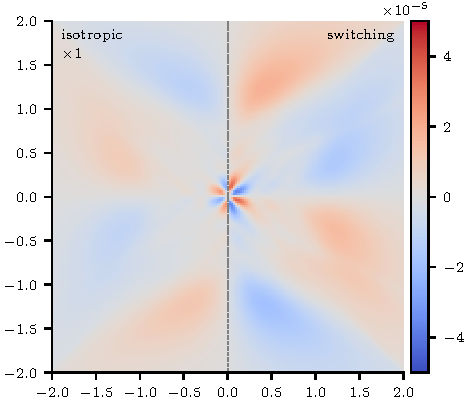
\includegraphics[width=\linewidth]{v-4r-4_uz_t_4}
      %\caption{$t=4$}
      %\label{fig:v-4r-4_uz_t_4}
    %\end{subfigure}
    \begin{subfigure}{0.32\textwidth}
      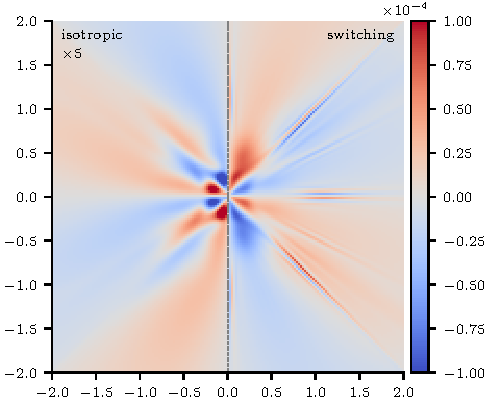
\includegraphics[width=\linewidth]{v-4r-4_uz_t_6}
      \caption{$t=6$}
      \label{fig:v-4r-4_uz_t_6}
    \end{subfigure}
    %\begin{subfigure}{0.32\textwidth}
      %\includegraphics[width=\linewidth]{v-4r-4_uz_t_8}
      %\caption{$t=8$}
      %\label{fig:v-4r-4_uz_t_8}
    %\end{subfigure}
    \begin{subfigure}{0.32\textwidth}
      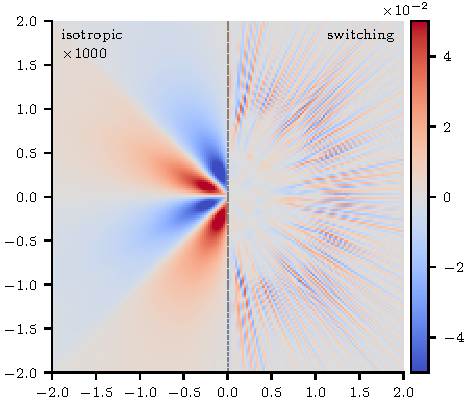
\includegraphics[width=\linewidth]{v-4r-4_uz_t_10}
      \caption{$t=10$}
      \label{fig:v-4r-4_uz_t_10}
    \end{subfigure}
    %\begin{subfigure}{0.32\textwidth}
      %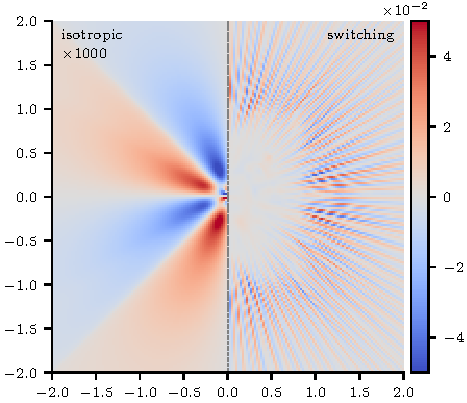
\includegraphics[width=\linewidth]{v-4r-4_uz_t_12}
      %\caption{$t=12$}
      %\label{fig:v-4r-4_uz_t_12}
    %\end{subfigure}
\caption{Out of plane velocity $u_z$ at $t=2, 6$ and $10$ for both viscosity models. Note the isotropic results have been multiplied by as much as $1000$ in order to compare to the switching results. In the switching case the KHI appears initially along the diagonals before extending azimuthally. In the isotropic case there is no evidence of the instability.}
\label{fig:out_of_plane_velocity}%
\end{figure}

Figure~\ref{fig:out_of_plane_velocity} shows the development of the out of plane velocity from $t=2$ to $10$. Both cases appear similar until $t=6$ when the KHI appears only in the switching case, initially along the diagonals (Figure~\ref{fig:v-4r-4_uz_t_6}) before spreading azimuthally (Figure~\ref{fig:v-4r-4_uz_t_10}). There is no evidence of the KHI in the isotropic case.

\subsubsection{Linear stability of the current-vortex sheet}

\begin{figure}[t]
  \centering
    \begin{subfigure}{0.49\textwidth}
      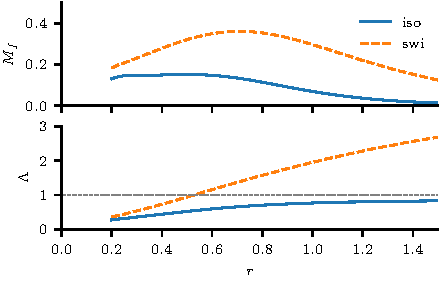
\includegraphics[width=\linewidth]{v-4r-4_mach_t_6}
      \caption{Stability parameters}%
      \label{fig:v-4r-4_mach_t_6}
    \end{subfigure}
    \hfill
    \begin{subfigure}{0.49\textwidth}
      \includegraphics[width=\linewidth]{v-4r-4_layers_with_time}
      \caption{Shear layer properties}
      \label{fig:v-4r-4_layers_with_time}
    \end{subfigure}
\caption{Properties of the shear layers for the isotropic case (blue, solid line) and switching case (orange, dashed line). Subfigure (a) plots the fast Mach number $M_f$ and stability measure $\Lambda$ as functions of radius $r$ at $t=6$. Subfigure (b) plots the dependence of the shear widths $L_u$ and $L_B$ and the shear magnitudes $\Delta u$ and $\Delta B$ as functions of time and at a radius of $r=0.7$. The major contributing factor to the instability of the shear layer in the switching case is the velocity shear.}
\label{fig:v-4r-4_layers}%
\end{figure}

Figure~\ref{fig:v-4r-4_mach_t_6} shows the relevant stability measures as functions of radius across the fan plane at $t=6$, a time when the fan plane has become unstable to the KHI in the switching case but remains stable in the isotropic case (Figure~\ref{fig:v-4r-4_uz_t_6}). The measure $\Lambda$ confirms that the current-vortex sheet is linearly stable to the KHI in the isotropic case and unstable in the switching case for $r>0.6$. This linear prediction matches where the KHI is observed to develop. In the switching case the peak of $M_f$ aligns with the observed region of initial growth of the instability.

Figure~\ref{fig:v-4r-4_layers_with_time} presents the thickness and magnitudes of the velocity and magnetic shear layers as functions of time. The magnetic shear layer appears relatively unaffected by the choice of viscosity model. In contrast, the lack of viscous damping in the switching case permits a thinner velocity shear layer with a magnitude that grows faster than in the isotropic case. This combination of a thinner, stronger velocity shear layer renders the current-vortex sheet unstable to the KHI while the damping effect of isotropic viscosity reduces the shear and suppresses the instability. The larger $\Delta u$ in the switching case is reflected in the stability measure $\Lambda$ (Figure~\ref{fig:v-4r-4_mach_t_6}).

The development of the magnetic shear layer is relatively unaffected by the viscosity 

\subsubsection{Breakup of the current-vortex sheet}

\begin{figure}[t]
  \centering
    \begin{subfigure}{0.48\textwidth}
      \includegraphics[width=\linewidth]{v-4r-4_vorticity_current_ring_t_10}
      \caption{Current-vortex sheet}
      \label{fig:v-4r-4_vorticity_current_ring_t_10}
    \end{subfigure}
    \hfill
    \begin{subfigure}{0.48\textwidth}
      \includegraphics[width=\linewidth]{v-4r-4_reconn_rate_t_10}
      \caption{Reconnection rate}
      \label{fig:v-4r-4_reconn_rate_t_10}
    \end{subfigure}
\caption{The breakup of the current-vortex sheet and associated reconnection at $t=10$. Subfigure (a) presents the current and vorticity density and subfigure (b) presents the spatial distribution of reconnection rate. Both subfigures show both viscosity models. The current-vortex sheet remains stable in the isotropic case while that in the switching case has been fragmented by the KHI. The resultant small-scale reconnection in the rolls produce localised pockets of strong vorticity and current density.}
\end{figure}

In both cases the current-vortex sheet grows in radius and magnitude with time, more in the switching case than in the isotropic. The shearing action of the counterflows produces a secondary ring of strong current density closer to the spine which is greater in magnitude in the isotropic case. By $t=10$ the KHI has disrupted the current-vortex sheet (Figure~\ref{fig:v-4r-4_vorticity_current_ring_t_10}) and the resultant rolls of the KHI create strong, small-scale current sheets, enhancing the local reconnection rate. 

Figure~\ref{fig:v-4r-4_reconn_rate_t_10} shows the spatial distribution of the reconnection rate for both viscosity models. Each pixel in the image represents one field line passing through that pixel along which the parallel electric field has been integrated. The colour of the pixel is given by the value of the integration. The reconnection rate is greatest close to the origin, corresponding to regions of slippage reconnection due to the strong currents in the spine and current-vortex sheet. The effects of the boundary can be seen as long dark lines which spiral outwards from the origin. The switching case shows greater peak reconnection rate due to the small scale current sheets created by the KHI, and the enhanced reconnection far from the null can be seen as ripple-like structures in the fringes of the plot.

\subsubsection{Spine-fan reconnection}

This section presents the results of driving a magnetic null to the point at which it undergoes spontaneous collapse. The collapse is instigated by a velocity shear across the null creating a magnetic shear which allows spine-fan reconnection. The results of the isotropic case are first presented in detail, then the effect of the KHI is explored in the switching case.

\begin{figure}[t]
  \centering
    \begin{subfigure}{0.49\textwidth}
      \includegraphics[width=\linewidth]{field_line_plots/cropped/v-4r-4-isotropic_0030_cropped.png}
      \caption{$t=15$}
      \label{fig:v-4r-4-iso-field-30}
    \end{subfigure}
    \hfill
    \begin{subfigure}{0.49\textwidth}
      \includegraphics[width=\linewidth]{field_line_plots/cropped/v-4r-4-isotropic_0037_cropped.png}
      \caption{$t=18.5$}
      \label{fig:v-4r-4-iso-field-37}
    \end{subfigure}
\caption{Collapse of the null point visualised with field lines. Field lines are plotted from a circle of radius $0.05$ around the upper and lower spine footpoints. Contours of $|\vec{j}| = 60$ are also plotted and reveal the strong current within the spine as well as the formation of the central sheet associated with the spine-fan reconnection. At $t=18.5$ the bulk of the field lines making up the core of the spines have reconnected.}
\label{fig:khi_field_lines_collapse}
\end{figure}

In typical studies of spine-fan reconnection (such as~\cite{pontinCurrentSheetFormation2007}) the spines of a null point are dragged in opposite directions at the boundaries. This motion pulls the field above and below the null point in opposite directions and creates a current sheet which acts to reconnect field lines between the spine and fan field lines. Here, the field near the null is shifted not because of motions at the footpoints of the spines, but due to imbalances in the velocity which arise naturally during the course of the initial driving. Figure~\ref{fig:khi_field_lines_collapse} presents the magnetic field lines before and during the reconnection.

\begin{figure}[t]
  \centering
    \begin{subfigure}{0.49\textwidth}
      \includegraphics[width=\linewidth]{v-4r-4-pressure-flow-30.pdf}
      \caption{Pressure and flow}
      \label{fig:v-4r-4-pressure-flow-30}
    \end{subfigure}
    \hfill
    \begin{subfigure}{0.32\textwidth}
      \includegraphics[width=\linewidth]{v-4r-4-vx-imbalance-30.pdf}
      \caption{Imbalance in $u_x$}
      \label{fig:v-4r-4-vx-imbalance-30}
    \end{subfigure}
\caption{Velocity imbalance above and below the null. Figure (a) plots a slice of the pressure through $y=0$ overlaid with fluid velocity, where the longest arrows correspond to a fluid velocity of approximately $0.1$. Figure (b) depicts $|u_x(x)| - |u_x(-x)|$, the difference in $u_x$ between the left and right sides of the plane $x=0$. This gives a measure of the asymmetry in the velocity around the null point.}
\label{fig:imbalance_in_velocity}
\end{figure}

The twist in the spines creates a current which heats the contained plasma via Ohmic heating and generates a small pressure force directed towards the null point. This drives two oppositely directed streams of plasma down the spines towards the null point (Figure~\ref{fig:v-4r-4-pressure-flow-30}). Where these streams meet at the null point, they form a stagnation point flow, compressing the plasma in the vicinity of the null and flowing out along the fan plane. Due to small asymmetries in the solution that accrue during the course of the simulation, an imbalance in the velocity appears above and below the null point (Figure~\ref{fig:v-4r-4-vx-imbalance-30}). 

\begin{figure}[t]
  \centering
    \begin{subfigure}{0.32\textwidth}
      \includegraphics[width=\linewidth]{v-4r-4-spine-fan-reconn-34.pdf}
      \caption{$t=17$}
      \label{fig:v-4r-4-spine-fan-reconn-34}
    \end{subfigure}
    \hfill
    \begin{subfigure}{0.32\textwidth}
      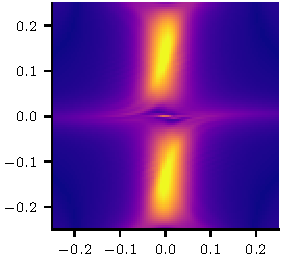
\includegraphics[width=\linewidth]{v-4r-4-spine-fan-reconn-35.pdf}
      \caption{$t=17.5$}
      \label{fig:v-4r-4-spine-fan-reconn-35}
    \end{subfigure}
    \hfill
    \begin{subfigure}{0.32\textwidth}
      \includegraphics[width=\linewidth]{v-4r-4-spine-fan-reconn-36.pdf}
      \caption{$t=18$}
      \label{fig:v-4r-4-spine-fan-reconn-36}
    \end{subfigure}
\caption{Development of the spine-fan reconnection current sheet shown as plots of $|\vec{j}|$ sliced through $y=0$ between $t=17$ and $18$. Maximum current density in all plots is $|\vec{j}| = 120$.}
\label{fig:spine_fan_reconnection_current_sheet}
\end{figure}

The velocity shear around the null shears the magnetic field accordingly, creating a current sheet through the null point in the process (Figures~\ref{fig:spine_fan_reconnection_current_sheet}). The current sheet enables reconnection between the spine and fan which further extends, thins and strengthens the sheet, continuing the reconnection process (Figure~\ref{fig:v-4r-4-iso-field-37}) until the field around the null collapses. The collapse itself can be seen in the kinetic energy as a dramatic increase starting at $t\approx18$ (Figure~\ref{fig:v-4r-4_kinetic_energy}). The development of the current sheet and the resultant spine-fan reconnection is similar to that of~\cite{pontinCurrentSheetFormation2007} with the exception that the twist in the field unravels as the reconnection proceeds. 

In the switching case, the development of the spine-fan reconnection and associated collapse is qualitatively similar to that in the isotropic case with the exception that the reconnection occurs notably earlier. Where the current sheet development shown in Figures~\ref{fig:spine_fan_reconnection_current_sheet} occurs between $t=17$ and $18$ in the isotropic case, a similar evolution occurs between $t=14$ and $15$ in the switching. This correlates 

\subsubsection{Overview of current-vortex sheet development and null collapse}

\begin{figure}[t]
  \centering
  \begin{subfigure}{0.32\textwidth}
    \includegraphics[width=\linewidth]{v-4r-4_kinetic_energy}
    \caption{Kinetic energy}
    \label{fig:v-4r-4_kinetic_energy}
  \end{subfigure}
  \hfill
  \begin{subfigure}{0.32\textwidth}
    \includegraphics[width=\linewidth]{v-4r-4_viscous_heating}
    \caption{Viscous heating}%
    \label{fig:v-4r-4_viscous_heating}
  \end{subfigure}
  \hfill
  \begin{subfigure}{0.32\textwidth}
    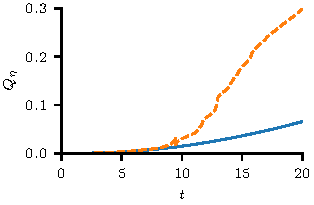
\includegraphics[width=\linewidth]{v-4r-4_ohmic_heating}
    \caption{Ohmic heating}%
    \label{fig:v-4r-4_ohmic_heating}
  \end{subfigure}
  \hfill
  \begin{subfigure}{0.32\textwidth}
    \includegraphics[width=\linewidth]{v-4r-4_magnetic_energy}
    \caption{Magnetic energy}%
    \label{fig:v-4r-4_magnetic_energy}
  \end{subfigure}
  \hfill
  \begin{subfigure}{0.32\textwidth}
    \includegraphics[width=\linewidth]{v-4r-4_internal_energy}
    \caption{Internal energy}%
    \label{fig:v-4r-4_internal_energy}
  \end{subfigure}
  \hfill
  \begin{subfigure}{0.32\textwidth}
    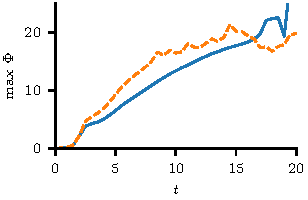
\includegraphics[width=\linewidth]{v-4r-4_reconn_rate_over_time}
    \caption{Reconnection rate}%
    \label{fig:v-4r-4_reconn_rate_over_time}
  \end{subfigure}
  \caption{Energy measures and reconnection rate as functions of time.}
  %\caption{Kinetic energy (a) and reconnection rate (b) as functions of time for the isotropic (blue, solid line) and switching (orange, dashed line) cases using diffusion parameters $\nu=10^{-4}$ and $\eta=10^{-4}$. The switching case shows clear growth of the KHI starting from $t=2$. While the isotropic case shows no evidence of the KHI, there is evidence of the null collapse at $t\approx18$. The reconnection rate reveals the nonlinear phase of the KHI as a period of bursty reconnection in the switching case and the eventual collapse in both cases.}
\end{figure}

\todo{replot energy and reconn rate once sims are complete}

The kinetic energy in the switching case reveals the main evolution of a KHI-unstable current-vortex sheet (Figure~\ref{fig:v-4r-4_kinetic_energy}). Initially, two torsional Alfv\'en waves are injected into the upper and lower spines of the null by the drivers. Due to viscosity and resistivity, the waves diffuse as they travel down the spine and along the fan plane, meeting at some radius and forming a current-vortex sheet at $t\approx3$. As the null continues to be driven, the sheet becomes unstable to the KHI and the kinetic energy grows accordingly. At $t\approx 8$ the KHI saturates as small-scale current sheets are formed and Ohmic heating begins to drain the energy from the instability (Figure~\ref{fig:v-4r-4_ohmic_heating}). This is also reflected in the reconnection rate, Figure~\ref{fig:v-4r-4_reconn_rate_over_time}, where the small current sheets in the fan plane 

After the formation of the current-vortex layer, it becomes unstable to the KHI only in the switching case. The total kinetic energy reveals the main developments of the instability (Figure~\ref{fig:v-4r-4_kinetic_energy}). The initial acceleration of the drivers and injection of torsional Alfv\'en waves occurs between $t=0$ and $2$. Then, the energy associated with the KHI grows only in the switching case, peaking at $t\approx 8$. Considering for a moment only the switching case, the instability generates vortices in the fan plane, encouraging current formation and enhanced Ohmic heating which in turn results in a drop of kinetic energy between $t=8$ and $10$ as the kinetic energy is converted to heat. Over the same time period, the isotropic case remains stable. The fast increases in kinetic energy around $t\approx 15$ in the switching case and $t\approx 18$ in the isotropic case signify the collapse of the null, discussed later.

\subsection{Analysis of parameter study}

The results shown in section~\ref{sec:null_point_khi_single_case} do not dramatically change when the viscosity $\nu$ is varied. However, the value of $\eta$ has a strong impact on the dynamics of the stressed null. Generally, increasing $\eta$ to $10^{-3}$ produces a null that remains unstable to the KHI (when using switching viscosity) but shows no sign of collapse. In contrast, decreasing $\eta$ to $10^{-5}$ causes the null to collapse much sooner than in the example case in section~\ref{sec:null_point_khi_single_case}, so much so that the KHI doesn't have time to develop nonlinearly, even in linearly unstable cases. We present first the quantitative effect of varying $\nu$, $\eta$ and the viscosity models on the properties of the shear layers and the resulting stability and development of the KHI. We then focus our analysis on the effect of only $\eta$ on the fluting instability and the null collapse, still comparing the two viscosity models.

%As an aside, in all $\nu = 10^{-3}$ isotropic simulations there's an unexpected, transient artifact in every examined variable. This was also seen in the kink instability simulations in chapter TODO. This is assumed to be due to small-amplitude fast waves created during the initial ramp up, the interaction of which causes the isotropic viscous stress tensor to produce odd effects. It appears to only affect the first time step and the effect is only to slightly increase the viscous heating. Since the affected results don't differ wildly from those of the unaffected $\nu=10^{-4}$ simulations we cautiously trust these results.

\subsubsection{Shear layer properties and instability}

To understand the effect that viscosity and resistivity have on the stability of the current-vortex sheet, it is useful to understand how changing their strength affects the thickness and magnitude of the vorticity and current density rings. After presenting an analysis of how these shear layer properties change with $\nu$ and $\eta$, the stability of these layers is presented and compared to predictions from the theoretical measures of stability introduced in section~\ref{sec:stability_measures}. The overall effect of viscosity and resistivity is to diffuse the upper and lower Alfv\'en waves as they travel through the null before meeting and diffusing in the fan plane, forming the shear layers that make up the current-vortex sheet. 

\begin{figure}[h]
  \centering
  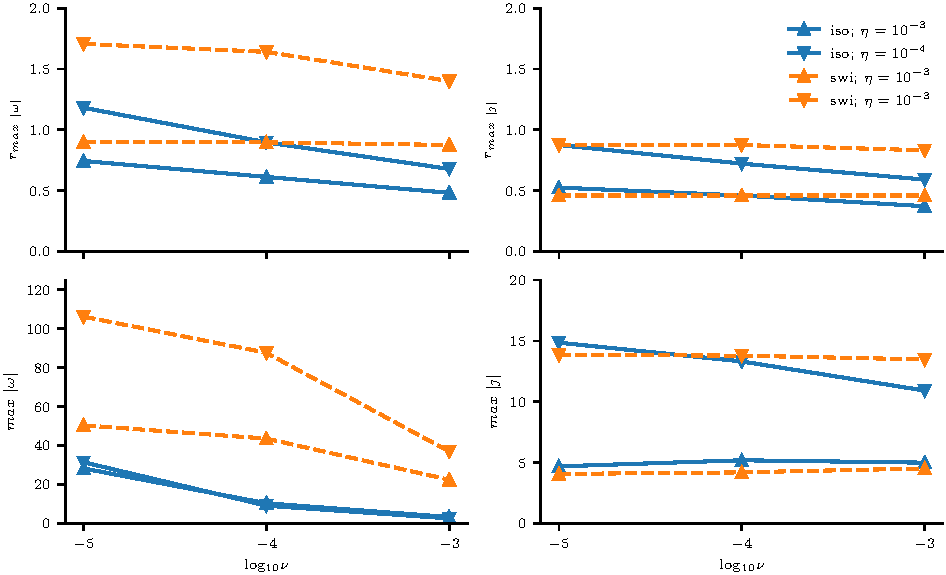
\includegraphics[width=\linewidth]{param_study/peak_mag_and_loc.pdf}
  \caption{Peak vorticity and current and the radii at which the peaks occur as functions of $\nu$ for each value of $\eta$ at $t=8$. The symbols represent $\eta=10^{-3}$ (downward-facing triangle) and $\eta=10^{-4}$ (upward-facing triangle) and the line styles represent the form of viscosity used, either isotropic (blue, solid lines) or switching (orange, dashed lines). In the isotropic case, both rings decrease in radial extent as either diffusion parameter is increased. In the switching case, both rings also decrease with $\eta$, however there is a notable increase in the radial extent with $\nu$, particularly for high values of $\eta$.}%
  \label{fig:param_study_peak_mag_and_loc}
\end{figure}

Figure~\ref{fig:param_study_peak_mag_and_loc} presents the peak vorticity and current density as functions of $\nu$ for both values of $\eta$, also plotting the radii at which the peaks occur. Increased diffusion leads to a thicker, weaker ring with a smaller radius. This is reflected in the general trends found in figure~\ref{fig:param_study_peak_mag_and_loc}, where peak current, peak vorticity and the radii at which the peaks occur all decrease with both diffusion parameters. The switching model, being generally less diffusive than the isotropic model, permits velocity shear layers with much greater peak vorticity and radial extent. Due to the coupling between the magnetic field and the velocity in an Alfv\'en wave, the isotropic model appears to provide some diffusion to the magnetic field during the formation of the magnetic shear layer, resulting in a layer with weaker peak current and smaller radial extent, however the switching model affects the layer very little.

\begin{figure}[t]
  \centering
  \includegraphics[width=1.0\linewidth]{param_study/layer_thickness_and_shear.pdf}
  \caption{The thickness of the velocity and magnetic shear layers $L_u$ and $L_B$, respectively, and the difference in velocity $\Delta u$ and magnetic field $\Delta B$ across the layers as functions of $\nu$ for each value of $\eta$ at $t=8$. The values for the velocity and magnetic shear layers are calculated at the radius at which the peak vorticity and current density occur, respectively. Increased diffusion in the form of either resistivity or viscosity results in thicker shear layers. As $\nu$ increases $\Delta u$ decreases and $\Delta B$ increases.}%
  \label{fig:layer_thickness_and_shear}
\end{figure}

Figure~\ref{fig:layer_thickness_and_shear} presents a measure of the thickness, $L_u$ and $L_B$, and the magnitudes, $\Delta u$ and $\Delta B$, of the velocity and magnetic shear layers, respectively. The radius at which these values are measured is the radius at which the peak vorticity or current density is found (as reported in figure~\ref{fig:param_study_peak_mag_and_loc}). 

The thickness of the shear layers is a direct result of how the initial Alfv\'en waves diffuse as they travel towards the fan plane. As the diffusion in the system increases, the thickness of the shear layers increases correspondingly (figure~\ref{fig:layer_thickness_and_shear}). Since the switching model is less diffusive than the isotropic model, the shear layers are generally thinner using this model. The effect of viscosity on the differences of velocity and magnetic field across the shear layers is more complex. With increased viscous diffusion, velocity is diffused more efficiently and the velocity difference across the velocity shear layer is reduced. In contrast, with increased viscous diffusion, the magnetic field difference across the magnetic shear layer is increased. This is a direct result of the enhanced viscous diffusion causing the initial Alfv\'en waves to meet closer to the null.

The distance the Alfv\'en waves travel before meeting affects the magnetic shear layer in two ways. Firstly, when the Alfv\'en waves are allowed to travel far along the field before forming the shear layers, the magnetic field on either side of the shear has more time to diffuse and reduce in magnitude. The other effect is a little more involved. Consider the effect of sending a wave pulse along a cable. Without much tension in the cable, the pulse has a certain amplitude. With greater tension in the cable, the energy required to bend the cable is increased, so the same pulse (with the same energy) will not be able to bend the cable quite so much and the resultant wave will have a smaller amplitude. Since the magnetic field strength of this particular null increases linearly with distance from the origin, the magnetic tension increases too. Analogous to the wave travelling along a cable under higher-tension, the Alfv\'en wave which travels further along the increasing magnetic field will be reduced in amplitude, hence reducing the magnitude of the magnetic shear.

\begin{figure}[h]
  \centering
  
\includegraphics[width=\linewidth]{param_study/kinetic_energies.pdf}
  \caption{Kinetic energy against time for each parameter choice. Runs using isotropic viscosity are shown as blue (solid) lines and switching viscosity as orange (dashed) lines. The distinctive energy profile of the Kelvin-Helmholtz instability is apparent in all switching cases and in the single isotropic case corresponding to $\nu = 10^{-5}, \eta = 10^{-3}$ in subfigure (a). Reconnection associated with the collapse of the null is signalled by sharp spikes in the kinetic energy starting around $t\approx13$ in the $\eta = 10^{-4}$ cases, subfigures (d-f), particularly in the isotropic cases. An increase in $\nu$ damps the energy released during the KHI in the switching cases and totally suppresses the KHI in the isotropic cases.}%
  \label{fig:param_study_kinetic_energies}
\end{figure}

The observed stability of KHI in the fan plane is determined via inspection of the out of plane velocity for each parameter choice and is summarised for each parameter choice in table~\ref{tab:stability}. The velocity is inspected at $t=8$, before the onset of other phenomena such as the null collapse. The stability and nonlinear development is also reflected in the kinetic energies~\ref{fig:param_study_kinetic_energies}. Simulations using the switching model develop a kinetic energy profile which displays a growth and decay shape indicative of the KHI. A similar pattern is also seen in the single fully-unstable isotropic case, figure~\ref{fig:param_study_kinetic_energies}(a).

The kinetic energy profiles also reveal some interesting cases of marginal stability which are investigated further by inspecting the out of plane velocity for $t>8$. The isotropic case~\ref{fig:param_study_kinetic_energies}(b) is found to be stable at all times, yet shows KHI-like growth in the kinetic energy. The isotropic case~\ref{fig:param_study_kinetic_energies}(d) and the switching case~\ref{fig:param_study_kinetic_energies}(f) show similar kinetic energy profiles and, upon inspection, show signs of instability at $t=12$. The full development of the instability in both cases is interrupted by the collapse of the null.

\begin{table}[]
\centering
\begin{tabular}{llllll}
$\nu$    & $\eta$    & $Pr_m = \nu/\eta$ & Isotropic stability & Switching stability &  \\
\midrule
$10^{-3}$ & $10^{-3}$ & $1$ & Stable                 & Unstable                 &  \\
$10^{-4}$ & $10^{-3}$ & $0.1$ & Stable                 & Unstable                 &  \\
$10^{-5}$ & $10^{-3}$ & $0.01$ & Unstable                 & Unstable                 &  \\
$10^{-3}$ & $10^{-4}$ & $10$ & Stable                 & Marginally unstable                 &  \\
$10^{-4}$ & $10^{-4}$ & $1$ & Stable                 & Unstable                 &  \\
$10^{-5}$ & $10^{-4}$ & $0.1$ & Marginally unstable                 & Unstable                 & 
\end{tabular}
\caption{Stability in the isotopic and switching cases for different choices of $\nu$ and $\eta$. The magnetic Prandtl number Pr$_m$ is also stated. The isotropic model mostly results in stability while the switching model mostly results in instability. There are two marginally unstable cases where the instability does not have time to fully develop.}
\label{tab:stability}
\end{table}

To further explore the observed stability of the KHI, we investigate how $M_f$ and $\Lambda$ vary radially, and link this to the stability and growth of the KHI. As an indicator of the stability of the shear layer, we plot the Mach number associated with the fast-mode $M_f = \frac{\Delta u}{\sqrt{c_s^2 + c_A^2}}$, where $\Delta u$ is the difference in velocity over the shear layer, and $c_s$ and $c_A$ are the local sound and Alfv\'en speeds, respectively, as well as the parameter $\Lambda = \frac{L_B}{L_u}(M_{A, proj})^{2/3}$, where $L_B$ and $L_u$ are the widths of the respective magnetic and velocity shear layers, and $M_{A, proj}$ is the Alfv\'en velocity of the layer after removing the guide field, i.e. $M_{A, proj} = \frac{\Delta u \sqrt{\rho}}{\Delta B}$ (TODO reword this entire sentence). For the layer to be theoretically unstable to the KHI, $M_f < 2$ and $\Lambda > 1$. These properties are investigated at $t=8$, around the time of KHI onset where it occurs, but well before the breakup of the current-vortex sheet, allowing accurate measurement of $M_f$ and $\Lambda$.

\begin{figure}[h]
    \hfill
    \begin{subfigure}{0.49\textwidth}
      \centering
  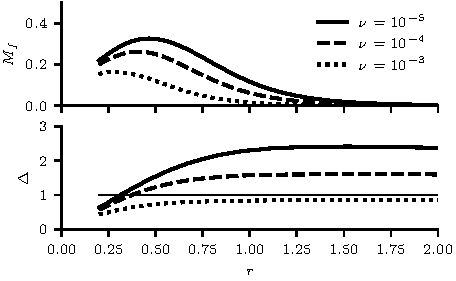
\includegraphics[width=1.0\linewidth]{param_study/mach_numbers_eta_3_iso.pdf}
      \caption{Isotropic; $\eta = 10^{-3}$}%
      \label{fig:mach_numbers_eta_3_iso}
    \end{subfigure}
    \hfill
    \begin{subfigure}{0.49\textwidth}
      \centering
  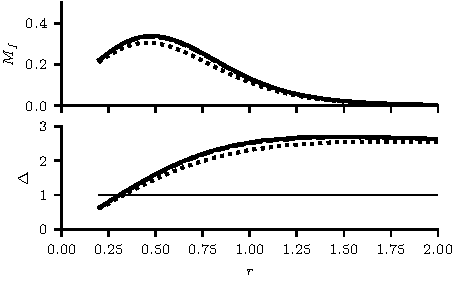
\includegraphics[width=1.0\linewidth]{param_study/mach_numbers_eta_3_swi.pdf}
      \caption{Switching; $\eta = 10^{-3}$}%
      \label{fig:mach_numbers_eta_3_swi}
    \end{subfigure}
    \hfill
    \begin{subfigure}{0.49\textwidth}
      \centering
  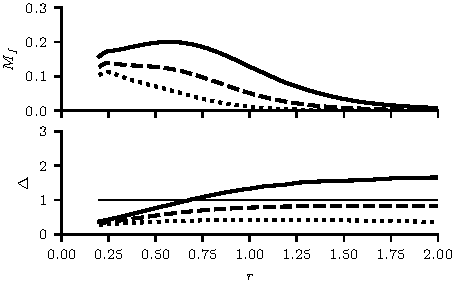
\includegraphics[width=1.0\linewidth]{param_study/mach_numbers_eta_4_iso.pdf}
      \caption{Isotropic; $\eta = 10^{-4}$}%
      \label{fig:mach_numbers_eta_4_iso}
    \end{subfigure}
    \hfill
    \begin{subfigure}{0.49\textwidth}
      \centering
  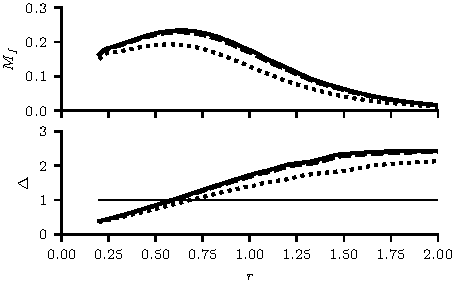
\includegraphics[width=1.0\linewidth]{param_study/mach_numbers_eta_4_swi.pdf}
      \caption{Switching; $\eta = 10^{-4}$}%
      \label{fig:mach_numbers_eta_4_swi}
    \end{subfigure}

  \caption{Plots of $M_f$ and $\Lambda$ as functions of $r$ for all parameter choices at $t=8$. Note the difference in the scale of $M_f$ for difference values of $\eta$. The cases where $\Lambda > 1$ are unstable with the exception of the isotropic cases where $\nu=10^{-4},\eta=10^{-3}$ (dashed line in figure~\ref{fig:mach_numbers_eta_3_iso}).}%
  \label{fig:mach_numbers}
\end{figure}

The observed stability summarised in table~\ref{tab:stability} is well matched by the theoretical conditions of instability, $\Lambda > 1$ and $M_f < 2$. Figure\ref{fig:mach_numbers} shows $M_f$ and $\Lambda$ plotted as functions of $r$ for each parameter choice. The condition $M_f < 2$ is satisfied in all runs, however the location of the peak of $M_f$ is where the current-vortex sheet is most unstable. Over all parameters, the maximum value of $M_f$ is less than $0.5$ suggesting the system would have to be driven at an unrealistically high velocity to approach the limit of $2$. The pertinent condition of instability for this particular presentation of the instability is thus $\Lambda > 1$. The simulations where this conditions is satisfied are unstable in all by one case, indicating that despite the difference in geometry and physics, the stability analysis of~\cite{einaudiResistiveInstabilitiesFlowing1986} is of practical use in predicting the stability of the KHI in magnetic null points. This condition even accurately predicts the stability of the marginal cases discussed previously. 

The isotropic case where $\nu=10^{-4},\eta=10^{-3}$ (dashed line in figure~\ref{fig:mach_numbers_eta_3_iso}) is the one outlier case where $\Lambda > 1$ over much of the current-vortex sheet, yet no instability is found in the out of plane velocity. The associated kinetic energy, figure~\ref{fig:param_study_kinetic_energies}(b), does show some initial growth, however this plateaus around $t\approx7.5$ and shows no further increase, unlike the kinetic energy of the marginally unstable isotropic case, figure~\ref{fig:param_study_kinetic_energies}(d), which continues to slowly increase. This suggests that the viscosity can affect stability not only by changing the thickness and magnitude of the current-vortex sheet as it forms, but also by stabilising a sheet which would otherwise be unstable. 

\begin{figure}[t]
  \centering
  \includegraphics[width=1.0\linewidth]{param_study/reconnection_rate.pdf}
  \caption{The reconnection rate max$\Phi$ as a function of time for each parameter choice. In all cases the reconnection rate increases with time due to slippage reconnection occurring throughout the null and within the magnetic shear layer. Where the KHI is excited, it encourages a greater rate of reconnection and causes the rate to temporarily dip around $t=10$, except in one case (subfigure (e)). Where $\eta=10^{-4}$ the isotropic cases show evidence of the reconnection rate dipping when the null collapses and the reconnecting current structures are disrupted, around $t=14$.}%
  \label{fig:khi_param_study_reconnection_rate}
\end{figure}

Figure~\ref{fig:khi_param_study_reconnection_rate} shows the reconnection rate over time for each parameter choice. Generally the switching model enhances the reconnection rate. This is due to the enhanced reconnection caused by the KHI, shown by the fact that the single fully-unstable isotropic case shares a similar reconnection rate profile (figure~\ref{fig:khi_param_study_reconnection_rate}(a)). When the KHI goes fully unstable, around $t=10$, the reconnection rate dips, except in the case of figure~\ref{fig:khi_param_study_reconnection_rate}(e) where the reconnection rate is significantly, transiently enhanced. The dip in reconnection rate coincides with a dip in kinetic energy (figure~\ref{fig:param_study_kinetic_energies}), indicating this is the point at which the KHI fully disrupts the current-vortex sheet, stalling the growth of the KHI and reducing the slippage reconnection which was occurring within the current ring. The case of the increase in reconnection rate in figure~\ref{fig:khi_param_study_reconnection_rate}(e) can be explained by noting that the break up of the current-vortex sheet is likely somewhat turbulent and could create transient current sheets capable of a high reconnection rate. The reconnection rate may be temporally under-resolved in this case. In the isotropic cases where $\eta=10^{-4}$ (figures~\ref{fig:khi_param_study_reconnection_rate}(d-f)) the collapse of the null is revealed in the reconnection rate, where the rate begins to dip at $t=14$.

Just as is found in the single case shown in section~\ref{sec:null_point_khi_single_case}, the simulations where $\eta = 10^{-4}$ show signs of collapse of the null starting around $t=13$, indicated by a sudden, bursty increase in kinetic energy~\ref{fig:param_study_kinetic_energies}(a-c), and the dip in the reconnection rate (figures~\ref{fig:khi_param_study_reconnection_rate}(d-f)) at $t=14$. The reason this occurs earlier in the parameter study simulations than in the higher resolution case in section~\ref{sec:null_point_khi_single_case} is because the lower resolution results in current structures compressing to the grid scale sooner, thereby setting off fast reconnection at an earlier time. 

\todo{add driver velocity param study? only stability I think}

\section{Discussion}
\label{sec:khi_discussion}

While the values of $\eta$ used in the simulations performed here are orders of magnitude greater than typical coronal estimates, the values of $\nu$ are certainly within realistic bounds. It has been found that, when using a model of viscosity appropriate in the solar corona, i.e. the switching model, the KHI is unstable, regardless of parameter choice. This strongly suggests that, in the real corona, the KHI can be excited in current-vortex sheets such as those studied here. What this investigation does not take into account are other possible null point configurations.

This chapter details the investigation of the KHI and null point collapse around an axisymmetric, linear null point, an idealised model of a real null point (such as that observed in~\cite{massonNATUREFLARERIBBONS2009}). The impact of non-ideal null configurations such as those with asymmetry (e.g. those investigated in~\cite{thurgoodImplosiveCollapseMagnetic2018,pontinWhyAreFlare2016a}) is unclear and is a valid avenue of further research. Similarly, the simplicity of the driver used here is unlikely to reflect the true nature of drivers in the real solar corona. The impact of driver complexity on spine-fan reconnection specifically has been investigated~\cite{wyperSpinefanReconnectionInfluence2012}, however the drivers studied in~\cite{wyperSpinefanReconnectionInfluence2012} only sheared the field (as opposed to the torsional drivers employed here). 

\todo{What about the speed of the driver? can slow drivers induce tearing?}

The simulations detailed in this chapter have been performed with a model of anisotropic viscosity which only captures the parallel component of viscosity. As discussed in~\cite{einaudiResistiveInstabilitiesFlowing1989}, the perpendicular components can become significant in strong velocity shears (such as those found in section~\ref{sec:khi_results}) despite the small size of the coefficient of perpendicular viscosity $\eta_1$ (see section~\ref{sec:braginskii_tensor}). A similar set of experiments exploring the effect of the perpendicular viscosity could provide useful insight, particularly in ascertaining whether the growth of the tearing instability could be accelerated by perpendicular viscosity, as is found in the linear analysis performed by~\cite{einaudiResistiveInstabilitiesFlowing1989}.

\todo{discuss tearing mode where KHI is stable}

An important, unexpected finding of this investigation is the spontaneous collapse of the null point without shearing drivers (as in~\cite{pontinCurrentSheetFormation2007}) or prescribed current density perturbations (as in~\cite{thurgoodImplosiveCollapseMagnetic2018}). The primary drivers of the shearing motion above and below the null (which gives rise to a current sheet, associated spine-fan reconnection and eventual collapse) are the oppositely directed streams of plasma flowing along the spines towards the null. These flows rely on the pressure gradients which are generated by Ohmic heating in the twisted spines. In chapter~\ref{chp:kink_instability_straight} it was found that the pressure generated in the ideal case (i.e. without any Ohmic heating) was too small to generate a fluting instability. Similarly, here, it may be that the pressure generated under ideal conditions (or using realistically small coronal resistivity) is not enough to drive the null-directed flows and, thus, not enough to collapse the null. Further investigation of this form of collapse within a twisted null point is required to ascertain if such a collapse is possible in the real corona.

The effect of the form of viscosity on the collapse of the null is also explored in the two high-resolution simulations (of Section~\ref{sec:null_point_khi_single_case}) and it is found that in the switching case, where the KHI is unstable, the null collapses notably earlier than in the isotropic case, where the KHI is stable. It is unclear if the early null collapse is a consequence of the KHI or the use of the switching model. From the results of the isotropic case, the null collapse appears to be ultimately caused by slight asymmetries in the spine-aligned flows, so one may conjecture that, in the switching case, the KHI introduces its own asymmetries which cause the early collapse of the null. A higher resolution version of the unstable, isotropic case (where $\nu = 10^{-5}$ and $\eta=10^{-3}$) would provide clarity and provides an avenue of further study.

It is unclear how the unravelling of the null as it collapses affects the ability of the null to undergo the kind of oscillatory reconnection found in~\cite{thurgoodThreedimensionalOscillatoryMagnetic2017}. One observed phase in the oscillatory process is the generation of back-pressure which halts and reverses the spine-fan reconnection process. It may be that a collapsing twisted null is unable to produce the required back-pressure if it unravels during its initial collapse. Running the high-resolution simulations reported here for a longer time would reveal if the particular setup studied here can generate oscillatory spine-fan reconnection. Alternatively, using a pre-twisted null point as an initial condition with the perturbation used to collapse the null found in~\cite{thurgoodThreedimensionalOscillatoryMagnetic2017} would provide a similar experiment.

The effect of the boundaries is very apparent.

%In the simulations performed here, the resolution was set such that the same number of grid points were used in each direction. In hindsight, the resolution could have been better balanced by using more grid points in the relatively long $x$ and $y$ directions than the relatively short $z$ direction, although this would have impacted the resolution across the shear layers. A non-uniform grid could have been used, with higher resolution focused near the null point. This is commonly done in other studies of null point dynamics~\cite{wyperKelvinHelmholtzInstabilityCurrentvortex2013,thurgoodThreedimensionalOscillatoryMagnetic2017}.

\section{Conclusions}
\label{sec:khi_conclusions}

In this chapter I have compared two models of viscosity applied to a magnetic null point which has been dynamically twisted at its footpoints in such a way that a current-vortex sheet forms in the fan plane. This sheet has the potential to become unstable to the KHI. It was found that increased viscous dissipation, particularly in the form of isotropic viscosity, has a stabilising effect on the sheet. This is primarily due to viscosity thickening the sheet and increasing its stability. The presence of the instability enhances reconnection locally within the sheet.
